\documentclass[sigconf]{acmart}
\usepackage{float}

\AtBeginDocument{%
  \providecommand\BibTeX{{%
    \normalfont B\kern-0.5em{\scshape i\kern-0.25em b}\kern-0.8em\TeX}}}

% 1. Title and Authors
\title{Competitive Esports Network: A Relational Approach to Tournament Management}

\author{Nastia Kossiak}
\affiliation{%
  \institution{University of Idaho}
  \city{Moscow}
  \state{Idaho}
  \country{USA}}

\author{Wyatt Fischer}
\affiliation{%
  \institution{University of Idaho}
  \city{Moscow}
  \state{Idaho}
  \country{USA}}

\author{Brandon Lunney}
\affiliation{%
  \institution{University of Idaho}
  \city{Moscow}
  \state{Idaho}
  \country{USA}}

\begin{document}

\begin{abstract}
This paper presents the design and implementation of the Competitive Esports Network, a relational database system developed to model interactions between players, professional teams, and tournaments. Using MySQL to manage the database, Python for backend management, and Cytoscape for visualization. The purpose of this database is to analyze the player network and participation patterns within tournaments and teams through queries.
\end{abstract}

% 3. CCS Concepts
\begin{CCSXML}
<ccs2012>
   <concept>
       <concept_id>10002951.10002952.10003190</concept_id>
       <concept_desc>Information systems~Relational databases</concept_desc>
       <concept_significance>500</concept_significance>
   </concept>
   <concept>
       <concept_id>10010405.10010476.10011187</concept_id>
       <concept_desc>Applied computing~Computer games</concept_desc>
       <concept_significance>300</concept_significance>
   </concept>
 </ccs2012>
\end{CCSXML}

\ccsdesc[500]{Information systems~Relational databases}
\ccsdesc[300]{Applied computing~Computer games}

\keywords{Esports, Relational Databases, MySQL, Cytoscape, Network Visualization, Python}

\maketitle

% ER Diagram
\section{Entity-Relationship Diagram}
\begin{figure}[H]
  \centering
  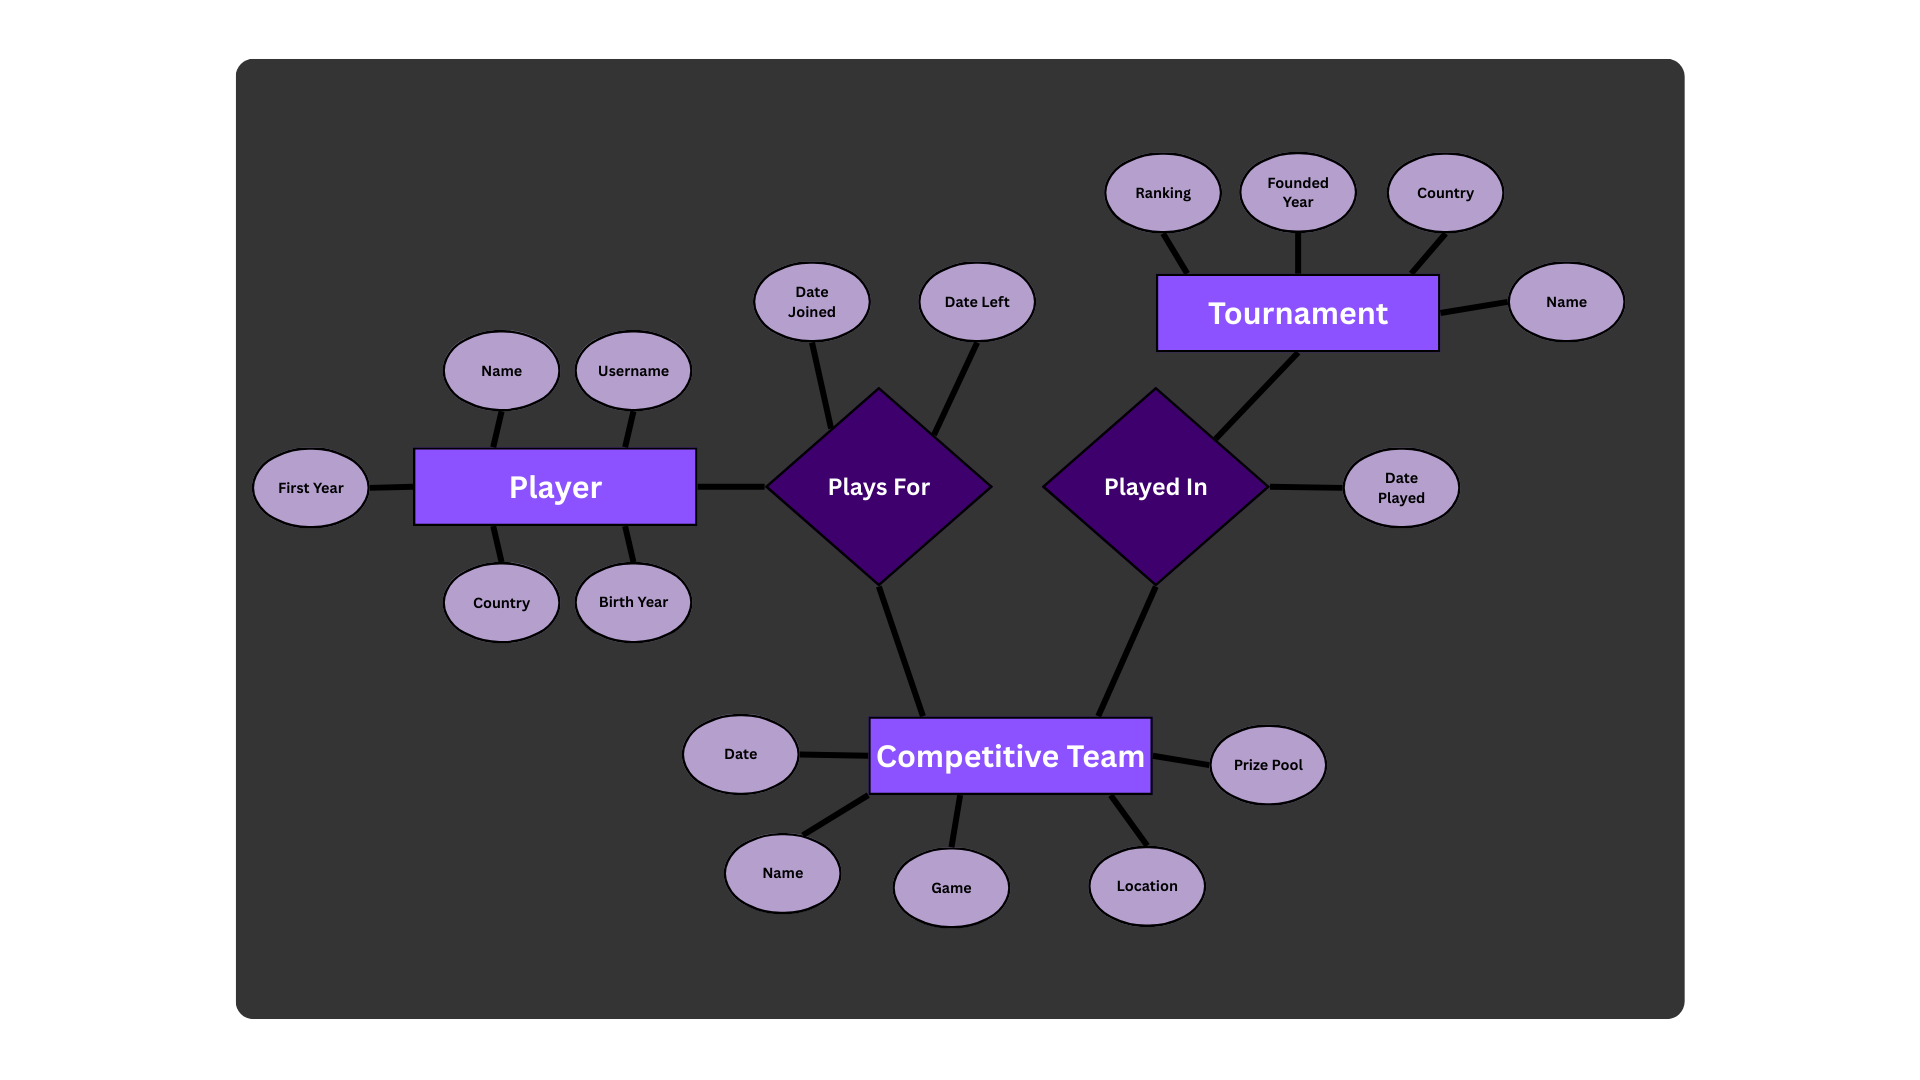
\includegraphics[width=\linewidth]{er} 
  \caption{ER Diagram for the Esports Network.}
  \label{fig:er}
\end{figure}

% ER Diagram
\section{Introduction}
The rapid growth of competitive gaming has created a need for robust data management systems. The Competitive Esports Network aims to map these relationships, focusing on three primary entities: Players, Competitive Teams, and Tournaments. 

\subsection{Understanding of Project}
The system represents players, teams, and tournaments as key nodes, while the relationships between them are modeled as edges. These relationships will show all the information such as which team a player belongs to, the change of teams over time, and their participation in tournaments. In addition, the model makes it possible so tournament statistics and placements for both teams and individual players are easy to determine based on these relationships. The system will be visualized in a graph based format.

\subsection{Interpretation of Requirements}
The requirements include a graph database system that supports different nodes, edge relationships, and queries ran over the resulting network. In our interpretation, the nodes are modeled as Player, Competitive Team, and Tournament entities, as shown in Figure~\ref{fig:er}. Relationships such as Plays For, Participates In, and Teammate represent interactions between these entities. There are required analytical queries, which we adapt to the Esports domain. The co-author query is interpreted as the teammate network visualization. The h-index style query is interpreted as identifying the players that participated on tournaments with high success. Finally, Q1 tournaments are defined dynamically by using a prize pool to represent different tiers of these events.

\section{Technology Stack}
Our implementation utilizes three different tools to build a technology stack that ensures data integrity and visual clarity.

\subsection{Database}
The core of the system is built on \textbf{MySQL}. We have developed an Entity-Relationship (ER) model that defines the relationship between players, their respective organizations, and the tournaments they have participated in. Key relationships include:
\begin{itemize}
    \item \textit{Plays For}: Mapping players to teams.
    \item \textit{Played In}: Connecting teams to specific tournament events.
\end{itemize}

\subsection{Backend}
We leverage \textbf{Python} for back-end logic and data processing. With this being one of the most widely used programming languages, we will be able to leverage our familiarity as well as extensive resources in implementing our project objectives.

\subsection{Visualization Tools}
To provide a graphical representation of the network, we integrate \textbf{Cytoscape}, allowing for advanced visualization of player-team-tournament nodes.  With the recent uptick in popularity among our working cohort, this tool will integrate flawlessly with the intent of this project.

\section{Project Plan}
The plan for this project is to gain a general understanding of all of the tools we have chosen in order to build skill sets related to building and leveraging databases.  We will spend the first portion of our time familiarizing ourselves with the tool and ensuring that our understanding of the requirements is correct.  We will then build out a prototype that will allow us to gain feedback on our implementation.  Building on the previous skills we have obtained we will finish out a working prototype with full documentation.  Based on the feedback we receive at this point, we will finish our database project.  I final demo of our work will finish out this project at the end of the 2026 Spring Semester.


\section{Timeline of Deliverables}
The development of this network is divided into four distinct phases:
\begin{description}
    \item[Phase I:] Initial design and requirement gathering.
    \item[Phase II:] Expansion of general design and basic prototype development.
    \item[Phase III:] Expansion design further and fully functional prototype development.
    \item[Phase IV:] Final report and system demonstration.
\end{description}

\section{Conclusion}
The Competitive Esports Network provides a scalable solution for managing the vast datasets generated by modern professional gaming. Using our relational database, an interested party will be able to gain valuable insights about the landscape of competitive gaming.  This expansion of understanding will be able to speed up the process of increasing an organization's competitive edge as well as talent acquisition.

\bibliographystyle{ACM-Reference-Format}
\begin{thebibliography}{9}

\bibitem{mysql}
MySQL Documentation. \\
\url{https://dev.mysql.com/doc/}. Accessed 2026.

\bibitem{cytoscape}
Cytoscape: An Open Source Platform for Complex Network Analysis and Visualization. \\
\url{https://cytoscape.org/}

\end{thebibliography}
\end{document}